\usepackage{amsthm}
\usepackage{mathtools}
\usepackage{physics}
\usepackage{calligra}
\usepackage{csquotes}
\usepackage{tensor}
\usepackage[thicklines]{cancel}
\usepackage{tcolorbox}
\usepackage{pstricks}
\usepackage[backend=biber, bibstyle=nature, sorting=nty, citestyle=numeric-comp]{biblatex} %Custom bibliography
    \addbibresource{bib.bib} %Load references


\DeclareMathAlphabet{\mathcalligra}{T1}{calligra}{m}{n}
\DeclareFontShape{T1}{calligra}{m}{n}{<->s*[2.2]callig15}{}
\newcommand{\scriptr}{\mathcalligra{r}\,}
\newcommand{\boldscriptr}{\pmb{\mathcalligra{r}}\,}
\def\rc{\scriptr}
\def\brc{\boldscriptr}
\def\hrc{\hat\brc}
\newcommand{\ie}{\emph{i.e.}} %id est
\newcommand{\eg}{\emph{e.g.}} %exempli gratia
\newcommand{\rtd}[1]{\ensuremath{\left\lfloor #1 \right\rfloor}}
\newcommand{\dirac}[1]{\ensuremath{\delta \left( #1 \right)}}
\newcommand{\diract}[1]{\ensuremath{\delta^3 \left( #1 \right)}}
\newcommand{\e}{\ensuremath{\epsilon_0}}
\newcommand{\m}{\ensuremath{\mu_0}}
\newcommand{\V}{\ensuremath{\mathcal{V}}}
\newcommand{\prnt}[1]{\ensuremath{\left(#1\right)}} %parentheses
\newcommand{\colch}[1]{\ensuremath{\left[#1\right]}} %square brackets
\newcommand{\chave}[1]{\ensuremath{\left\{#1\right\}}}  %curly brackets

\useoutertheme{infolines}
\useinnertheme{rectangles}
\usefonttheme{professionalfonts}


\definecolor{orange}{HTML}{f28165}
\definecolor{gray}{HTML}{303030}
\definecolor{yellow}{HTML}{f0be52}
\definecolor{lightorange}{HTML}{f19e58}

\renewcommand{\CancelColor}{\color{orange}}

\makeatletter
\newcommand{\mybox}[1]{%
  \setbox0=\hbox{#1}%
  \setlength{\@tempdima}{\dimexpr\wd0+13pt}%
  \begin{tcolorbox}[colback=orange,colframe=orange,boxrule=0.5pt,arc=4pt,
      left=6pt,right=6pt,top=6pt,bottom=6pt,boxsep=0pt,width=\@tempdima]
    \textcolor{white}{#1}
  \end{tcolorbox}
}
\makeatother

\usecolortheme[named=orange]{structure}
\usecolortheme{sidebartab}
\usecolortheme{orchid}
\usecolortheme{whale}
\setbeamercolor{alerted text}{fg=yellow}
\setbeamercolor{block title alerted}{bg=alerted text.fg!90!black}
\setbeamercolor{block title example}{bg=lightorange!60!black}
\setbeamercolor{background canvas}{bg=gray}
\setbeamercolor{normal text}{bg=gray,fg=white}

\setbeamertemplate{footline}
        {
      \leavevmode%
      \hbox{%
      \begin{beamercolorbox}[wd=.333333\paperwidth,ht=2.25ex,dp=1ex,center]{author in head/foot}%
        \usebeamerfont{author in head/foot}\insertshortauthor~~(\insertshortinstitute)
      \end{beamercolorbox}%
      \begin{beamercolorbox}[wd=.333333\paperwidth,ht=2.25ex,dp=1ex,center]{title in head/foot}%
        \usebeamerfont{title in head/foot}\insertshorttitle
      \end{beamercolorbox}%
      \begin{beamercolorbox}[wd=.333333\paperwidth,ht=2.25ex,dp=1ex,center]{date in head/foot}%
        \usebeamerfont{date in head/foot}\insertshortdate{}%\hspace*{2em}

    %#turning the next line into a comment, erases the frame numbers
        %\insertframenumber{} / \inserttotalframenumber\hspace*{2ex} 

      \end{beamercolorbox}}%
      \vskip0pt%
    }


\setbeamertemplate{blocks}[rectangle]
\setbeamercovered{dynamic}

\setbeamertemplate{section page}
{
	\begin{centering}
		\begin{beamercolorbox}[sep=27pt,center]{part title}
			\usebeamerfont{section title}\insertsection\par
			\usebeamerfont{subsection title}\insertsubsection\par
		\end{beamercolorbox}
	\end{centering}
}

%\setbeamertemplate{subsection page}
%{
%	\begin{centering}
%		\begin{beamercolorbox}[sep=12pt,center]{part title}
%			\usebeamerfont{subsection title}\insertsubsection\par
%		\end{beamercolorbox}
%	\end{centering}
%}

\newcommand{\hlight}[1]{\colorbox{violet!50}{#1}}
\newcommand{\hlighta}[1]{\colorbox{red!50}{#1}}
\pdfinfo{
  /Creator (LaTeX)
  /Title   (TITLE)
  /Author  (AUTHOR)
}


\title{Elegance}
\subtitle{An elegant theme for Beamer}
\author{Ivan Čukić}

\institute{\color{white}
    email@address.org \\
    http://address.org
} %
\date{\footnotesize\color{mainthemecolour} Conference, City 2016. }



\begin{document}

\maketitle


\section{Themes}

\subsection{Background images}

\begin{xframe}{Themes for the Elegance}

    You need a \hl{style/images} directory
    with these files inside:

    \begin{itemize}
        \item background-section.pdf
        \item background-slide.pdf
        \item background-title.pdf
        \item logo.png
    \end{itemize}

\end{xframe}


{
\usebackgroundtemplate{
\includegraphics[width=\paperwidth]{../screenshots/theme-1.png}}
\begin{frame}[plain]
    .
\end{frame}
}


{
\usebackgroundtemplate{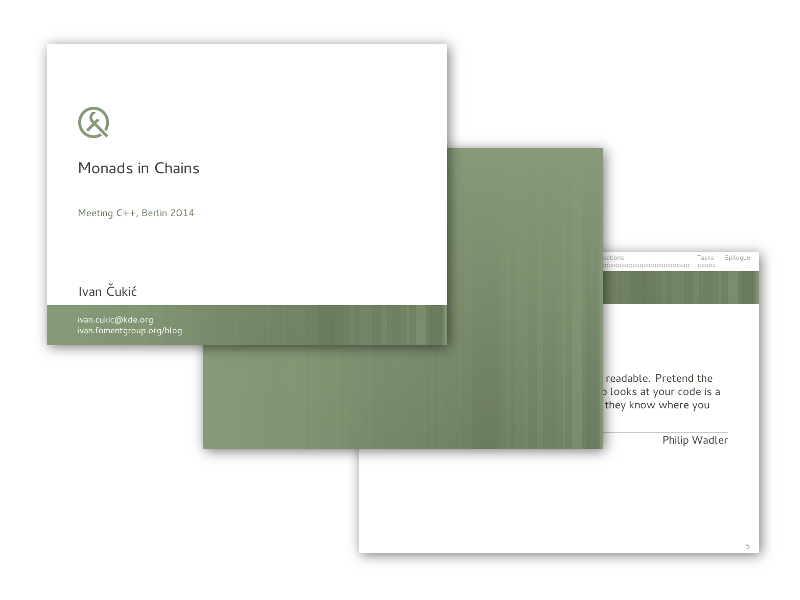
\includegraphics[width=\paperwidth]{../screenshots/theme-2.png}}
\begin{frame}[plain]
    .
\end{frame}
}


{
\usebackgroundtemplate{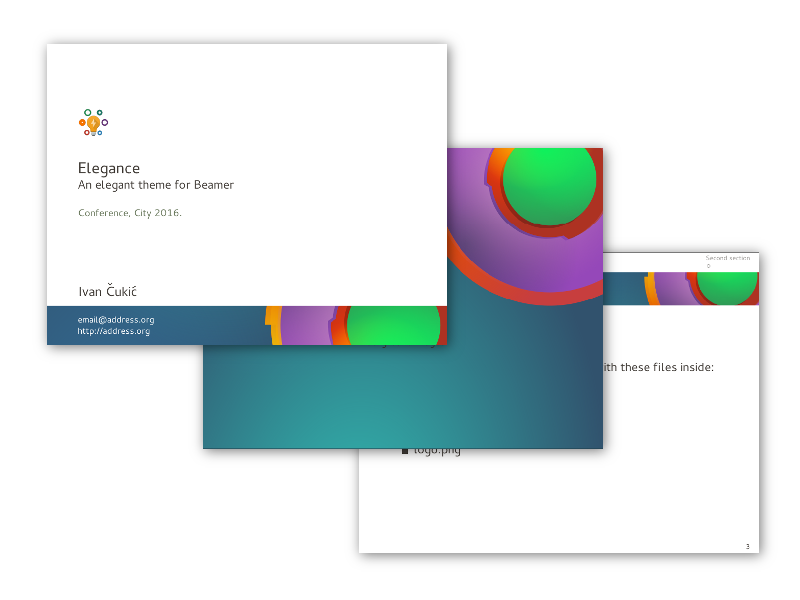
\includegraphics[width=\paperwidth]{../screenshots/theme-3.png}}
\begin{frame}[plain]
    .
\end{frame}
}





\section{Examples}

\subsection{Showing code}

\begin{xframe}{Code snippets}

    Do you have some code to show on the slide?

    And the same frame should also contain text?

    \begin{cxxcodebox}
        class example {
            // \codedots shows grayed-out dots
            @ \codedots @
        };
    \end{cxxcodebox}

    You can use \verb|cxxcodebox| environment.
    It has \verb|cxx| in the name,
    but no syntax highlighting is performed.

    For short code snippets,
    it is better just to highlight the important parts.

\end{xframe}


\subsection{Code slides and escapes}

\begin{xframe}{Second slide}

    \begin{cxxcode}
        class example {
            // There are a few useful escapes here
            @ \codedots @ // \codedots shows grayed-out dots

            // Invalid parts can be marked with \hlErr
            @\hlErr{operator;}@

            // Good parts can be marked with \hlOk
            @\hlOk{operator() ()}@

            // Other highlighting commands can be seen in
            // the preamble.tex file
        };
    \end{cxxcode}

\end{xframe}

\end{document}
